\chapter{Knowledge Enabled Situated Natural Language Processing}
\label{chapt|dialogs}

%%%%%%%%%%%%%%%%%%%%%%%%%%%%%%%%%%%%%%

\fxwarning{Mention and detail immanent communication -> context sharing}

\section{Grounding verbal interaction into the robot knowledge}
\label{sect|dialogs}

\subsection{Situated speech acts}
\label{intro_example}

A messy kitchen table, covered with knifes, spoons, bowls... Tom is preparing
the brownie, with Robi and Roba, its two robots.

`` -- Robi, give me this bowl'', says Tom, looking at the table. The robot
smoothly grasps the bowl, and hands it to the human.

What are the prerequisites for such a human sentence --- ``Robi, give me this
bowl'' --- to be understood by the robot, correctly interpreted in the spatial
context of the interaction, and ultimately transformed into an action?

Austin~\cite{Austin1962} would have at first glance analysed such kind of
sentence as a \emph{speech act}, comprising of \emph{locutionary},
\emph{illocutionary} and possibly \emph{perlocutionary} acts: First, we want to
understand the direct meaning of the sentence (\emph{locutionary act}): we must
acquire the sentence, convert it into a useful syntactic form (quite probably
by mean of speech recognition), and understand the semantics of the sentence,
\ie What is referred by ``\textit{Robi}''? What is ``\textit{give}''? What is
``\textit{me}''? And ``\textit{this bowl}''?

Working in a situated context, we want furthermore to \emph{resolve} these
semantics atoms (\ie ground them) in the sensory-motor space of the robot. For
instance, ``\textit{this}'' is a demonstrative pronoun that refers in this
context to the object the human is focusing on, whatever \textit{focusing}
means: here, we guess Tom is looking at some bowl, which is a
possible cue. But it could as well point at something or refer to some
previously mentioned concept.

\begin{figure}%[!ht] 
    \centering
    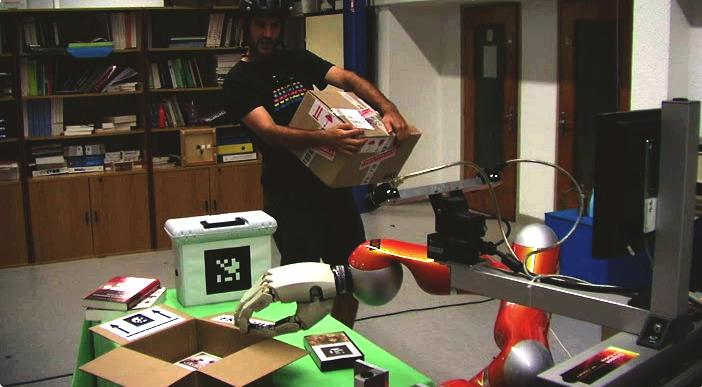
\includegraphics[width=0.9\linewidth]{images/dialogs/pt.jpg}
    \caption{Asking the robot to hand over a tape on the table.}
    \label{fig|vpt}
\end{figure}

Second, the \emph{illocutionary force}, \ie the \emph{intent} of the utterance
as thought by the agent must be extracted, and understood. In our example, Tom
obviously wants an action to be performed by the robot. The action
parametrisation is conveyed by the semantics attached to the words and the
grammatical structures of the sentence. In our example, the type of action is
given by the verb ``\textit{give}''. Assuming the robot has some procedural
knowledge (a planning domain and a planner) attached to this symbol, the action
type can be considered as grounded for the robot. We can as well understand
that the recipient of the action is the human, the performer is the robot
itself, and the object acted upon is the bowl. These are the basic
\emph{thematic roles} that can be extracted from the sentence that allow to
fully ground the action.

Extracting these speech acts and turning them into a content processable by the
robot is a difficult challenge in the general case. We base our approach on
three distinct, inter-related cognitive functions:

\begin{inparaenum}[\itshape 1)]

\item \emph{Physical environment modelling} and \emph{spatial reasoning}
(grouped under the term \emph{situation assessment})  are in charge of building
and maintaining a coherent model of the physical world. We have presented SPARK
in the previous chapter.

\item \emph{Knowledge representation and management}: we have also already
presented the ORO server in the previous chapters. It endows the robot with an
active knowledge base that provides a logically sound symbolic model of its
beliefs on the world, as well as models for each cognitive agent the robot
interacts with.

Used in combination with the situation assessment framework, the robot is thus
able to maintain different models of the world, one per agent. This proves an
essential feature~\cite{Roy2005, Kruijff2010} to enable perspective-aware
grounding of natural language, as we will see in next sections.

\item \emph{Dialogue input processing}, including natural language parsing
capabilities, disambiguation routines and interactive concept anchoring. We
focused our efforts on three classes of utterance, commonly found in
human-robot interaction: \emph{statements} (\ie new facts the human wants to
inform the robot), \emph{orders} (or more generically \emph{desires}) and
\emph{questions on declarative knowledge} (whose answers do not require
explicit planning). This would roughly cover the \emph{representative}
(sometimes referred as \emph{assertives}) and \emph{directives} type of
illocutionary acts in Searle~\cite{Searle1976} classification.

\end{inparaenum}

\subsection{Related work}
\label{sect|dialogs-related-work}

Processing natural language in situated context is already an established
research field. We have already mentioned Roy and Reiter~\cite{Roy2005} that
propose cross-modal representation systems, association of words with
perceptual and action categories, modelling of context, figuring out the right
granularity of models, integrating temporal modelling and planning, the ability
to match past (learned) experiences with the current interaction and the
ability to take into account the human perspective as the main challenges of
situated dialogue processing.

Kruijff et al. provides in~\cite{Kruijff2010} an up-to-date survey of literature
on situated human-robot dialogue, focusing on formal representation systems,
bi-directionality of the interaction and context building. They point as well
that, compared to the cognitive psychology community, the ``situated AI''
community started only recently to take into account agents focus, perspective and temporal
projection abilities.

Dialogue processing on real robots have been explored by several teams.
Scheutz~\cite{Brick2007} has contributions regarding natural language
processing in an incremental way, and how this enables instant back-channel
feedback (like nodding).

Hüwel et al.~\cite{Huwel2006} propose the concept of \textit{Situated Semantic
Unit}: these meaning atoms are extracted from sentences and expose semantic
links to other units. The parser tries to satisfy these links and rate
accordingly the semantic interpretation of the sentence. Used in conjunction
with ontologies, their approach offers good robustness to ungrammatical or
partial utterances. They validated the approach with an extensive user-study.

\fxwarning{Kollar/Tellex}

Several other systems, already presented at chapter~\ref{chapt|krs}, have
tackled the challenge: the Tapas system, the GLAIR architecture, GSM or the Ke
Jia project.

Compared to these previous contributions, our efforts have two foci: {\it (1)}
integration between language processing and perception of the environment and
the humans, from several perspectives; and {\it (2)} realistic human-robot
interactions: real-time processing; open speech; complex, dynamic, partially
unknown human environments; fully embodied autonomous robots with manipulation
abilities. 

We do not claim however any significant contribution to the field of
theoritical computational linguists (see \cite{Kruijff2010} for a survey of
formal approaches to natural language processing in the robotics field): our
main contribution here is the grounding of concepts involved in the human
discourse through the robot's own knowledge.

Section~\ref{dialog} presents the overall grounding process and
section~\ref{examples} proposes an analysis of the processing of three
prototypical sentences.  Experimental results are presented in the next chapter
on the evaluation.

%%%%%%%%%%%%%%%%%%%%%%%%%%%%%%%%%%%%%
\section{The Natural Language Grounding Process}
\label{dialog}

As stated above, we process three categories of
sentences: \emph{statements}, \emph{desires} and \emph{questions} that can be
answered from the declarative knowledge present in the robot knowledge base (a
choice similar to the \emph{Behaviour Cycle} in the GLAIR
architecture~\cite{Shapiro2009}). In our work, the grounding process of the
human discourse consists in extracting either the \emph{informational} content
of the sentence to produce statements or its \emph{intentional} content (\ie
performative value) to collect orders and questions.

\begin{figure}[!ht]
\centering
  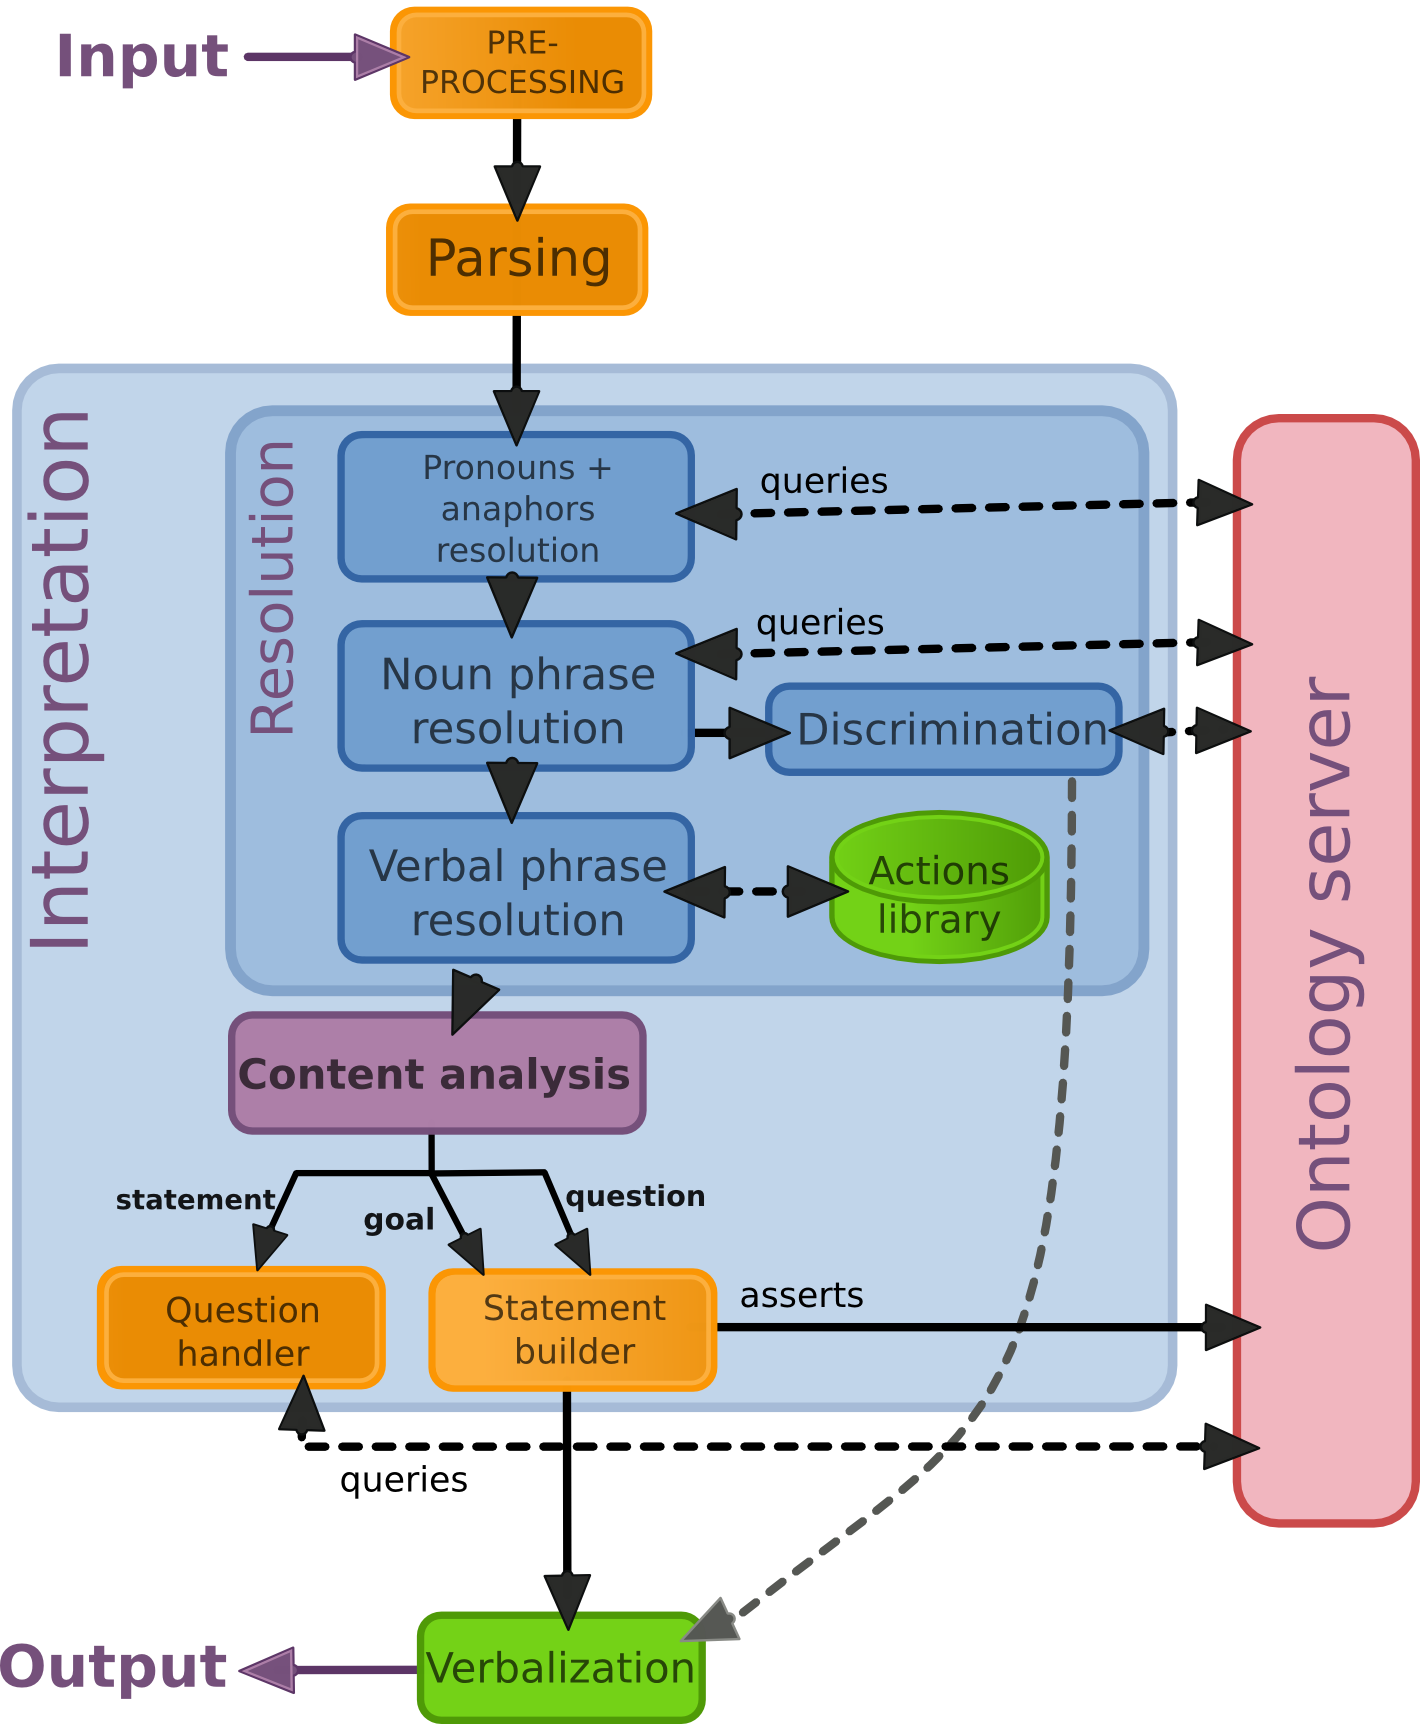
\includegraphics[width=0.6\linewidth]{images/dialogs/dialog_module_simple.pdf}

  \caption{The {\sc Dialogs} module has four main steps: the parsing, the
  resolution, the interpretation and the verbalisation.}

  \label{fig|dialog}
\end{figure}

As shown in Figure~\ref{fig|dialog}, the {\sc Dialogs} module that we have
developed, is composed of four main blocks. The user's input is first
pre-processed. For instance, \emph{I'm} constructs are expanded into \emph{I
am} and then parsed. The parser is a custom-made, rule-based (\ie grammar-free)
tool that extracts the grammatical structure from the user's sentence.

Figure~\ref{dialog|parser_output} shows an example of the raw output of the
parser for a moderately complex sentence.

\begin{figure}%[!ht]
\centering
\scriptsize
\begin{alltt}
>> IMPERATIVE
VP: \textbf{remember} (present simple)
    SUBSENTENCE (aim: that)
      NP: \textbf{I}
      VP: \textbf{want} (present simple)
        direct objects: 
          NP: \textbf{you}
        secondary VP: \textbf{give} ()
              direct objects:
                NP: my \emph{nice blue} \textbf{bottle}
              indirect objects:
                NP: \textbf{me}
\end{alltt}
\caption{Raw output of the {\sc Dialogs} parser after processing the
sentence: ``remember that I want you to give me my nice blue bottle.'' 
Nominal groups are not grounded yet.} 
\label{dialog|parser_output}
\end{figure}

The result of the parsing is then sent to the \emph{resolution} module.  The
processing can be divided again in three steps: {\it(1)} pronouns and anaphora
are replaced by, respectively, the correct speaker ID and the ID of the last
object spoken about (extracted from the dialogue history), {\it(2)} nominal
groups are disambiguated and grounded (noun phrase resolution), and {\it(3)}
verbal groups are resolved as well, and their associated thematic roles are
retrieved (verbal phrase resolution). Algorithm~\ref{algo|Resolution} describes
the overall process (with the subroutine \emph{GenerateDescription} presented
in algorithm~\ref{algo|generatedescription},
page~\pageref{algo|generatedescription}).  Next section describes specific
examples to show how the noun and verbal phrase resolution takes place.

\small
\begin{pseudocode}[ruled]{Resolution}{sentence, currentSpeaker}
\label{algo|Resolution}

\mathcal{G} \GETS \CALL{ParseNominalGroups}{sentence} \\

\FOREACH g \in \mathcal{G} \DO 
\BEGIN
   \mathcal{D} \GETS \CALL{GenerateDescription}{g} \STMTNUM{5.1em}{res.desc}\\
   candidates \GETS \CALL{Ontology.Find}{\mathcal{D}} \STMTNUM{4em}{res.onto}\\
   
   \IF \left|{candidates}\right| = 0 \THEN
    \BEGIN
      \OUTPUT{\mbox{Couldn't resolve the group!}} \\
      \EXIT \\
    \END
   \ELSEIF \left|{candidates}\right| = 1 \THEN
      id \GETS candidates[0] \STMTNUM{8em}{res.easy}\\

   \ELSE
      \BEGIN
        \IF \CALL{Ontology.CheckEquivalent}{candidates} \THEN
          id \GETS candidates[0] \\
        \ELSE
          id \GETS \CALL{Discrimination}{candidates, currentSpeaker} \\ %\STMTNUM{1em}{st.discrimination}\\
      \END \\
   \CALL{Replace}{g, id, sentence}
\END
\end{pseudocode}
\normalsize

The result of the resolution is then send over to the \emph{interpretation}
module that first performs a \emph{content analysis} (what was the intent of
the utterance: information, question or desire) and then translate the original
sentence into RDF statements (the \emph{statement building} step).

As represented in Figure~\ref{fig|dialog}, both resolution and interpretation
tightly rely on the communication with the knowledge base. All the concepts the
robot manipulates are stored in the ontology server and retrieved through
logical queries, except for the verbs that are currently stored in a dedicated
library (the \emph{action library} in the diagram).

\small
\begin{pseudocode}[ruled]{GenerateDescription}{group}
\label{algo|generatedescription}

\PROCEDURE{GenerateDescription}{group} 
   noun \GETS \CALL{GetNoun}{group} \\ 
   \IF \CALL{Ontology.Lookup}{noun} \in (Instances) %\STMTNUM{7.5em}{st.lookup} \THEN
   		\BEGIN
		id \GETS \CALL{Ontology.Lookup}{noun}\\	
		\RETURN {\mathcal{D} + \langle *\ {\tt sameAs}\ <id> \rangle}\\
		\END
   \ELSE
    	\mathcal{D} = \mathcal{D} + \langle *\ {\tt type}\ <noun>\rangle \\
   
   \\
   det \GETS \CALL{GetDeterminant}{group} \\
   \IF det \in {\mbox(possessives)} \THEN
       \mathcal{D} = \mathcal{D} + \langle *\ {\tt isRelatedTo}\ <possessor>\rangle \\
    
    \IF det \in {\mbox(demonstratives)} \THEN
        \BEGIN
        \IF \CALL{Ontology.Check}{\langle<currentSpeaker>\ {\tt focusesOn}\ *\rangle} \THEN 
            \mathcal{D} = \mathcal{D} + \langle<currentSpeaker>\ {\tt focusesOn}\ *\rangle
        \ELSE
            \mathcal{D} = \mathcal{D} + \CALL{AnaphoricMatching}{} %\STMTNUM{4em}{st.anaphoric} \\
        \END \\
   \\
   adjs \GETS \CALL{GetAdjectives}{group} \\
   \FOREACH adj \in adjs \DO
   	\BEGIN
   		\IF adj == ''other'' \THEN 
   			\BEGIN
   			id \GETS \CALL{History.GetMatchingConcept}{group} %\STMTNUM{8em}{st.history}\\
   			\mathcal{D} = \mathcal{D} + \langle *\ {\tt differentFrom}\ <id> \rangle\\
   			\RETURN{D}\\
			\END   		
   		\ELSE
	     	\mathcal{D} = \mathcal{D} + \langle *\ {\tt hasFeature}\ <adj>\rangle %\STMTNUM{9em}{st.adj} \\
    \END\\
    
   \\  
   nounCmplts \GETS \CALL{GetNounComplements}{group} \\
   \FOREACH cmplt \in nounCmplts \DO
     \mathcal{D} = \mathcal{D} + {\CALL{GenerateDescription}{cmplt}}\\
   
   
   \\  
   relativeClauses \GETS \CALL{GetSubordinateRelativeClauses}{group} \\
   \FOREACH relative \in relativeClauses \DO
   	\BEGIN
   	 \mathcal{G} \GETS \CALL{GetNominalGroups}{relative} \\
   	 \FOREACH g \in \mathcal{G} \DO
     	\mathcal{D} = \mathcal{D} + {\CALL{GenerateDescription}{g}}
    \END\\
     
   \\
   \RETURN{\mathcal{D}} 
\ENDPROCEDURE
\end{pseudocode}
\normalsize

\small
\begin{pseudocode}[ruled]{History.GetMatchingConcept}{group}
\label{algo|History}
\PROCEDURE{History.GetMatchingConcept}{group}
\COMMENT{Extract resolved nominal groups from sentences stored in the history}\\
\mathcal{H} \GETS \CALL{History.GetAllPastIds}{}\\
\COMMENT{The adjective  "other" is removed before recursively calling this routine} \\
	\mathcal{G} \GETS \CALL{Ontology.Find}{\CALL{GenerateDescription}{group}} \\ 
	
	candidates \GETS \mathcal{H} \cap \mathcal{G}\\
	\IF \left|{candidates}\right| = 0 \THEN
    \BEGIN
      \OUTPUT{\mbox{Couldn't find another object with the same characteristics!}} \\
      \EXIT \\
    \END
   \ELSEIF \left|{candidates}\right| = 1 \THEN
      id \GETS candidates[0]
   \ELSE
   	  id \GETS \CALL{Discrimination}{candidates}\\
   \RETURN{id}
\ENDPROCEDURE
\end{pseudocode}
\normalsize

%%%%%%%%%%%%%%%%%%%%%%%%%%%%%%%%%%%%%
\section{Technical analysis}
\label{examples}

In order to better understand the overall process of the {\sc Dialogs} module
and its relation with ORO, we next describe the different steps of the approach
based on three examples. In these examples we assume that some initial facts
are present in the knowledge base (either from initial common-sense knowledge
or through run-time acquisition), both in the robot's own model and in the
model of the human.  Since the robot tries to ground a human utterance, all
queries are sent to the human model in order to interpret it from the human
perspective.

\subsection{Informational Content Extraction}
\label{informational_content_extraction}

\begin{figure}
    \footnotesize
    \centering
%	\begin{tabular}{p{0.5\columnwidth} | p{0.5\columnwidth}}}
	\begin{tabular}{l|l}
	\emph{Initial knowledge} \texttt{human\_01} &
	\emph{Human input}\\	
	
	\hline

    	\stmt{banana\_01 type Banana} &
	``The yellow banana is big!'' \\
	
    	\stmt{banana\_01 hasColor yellow} & \\
	\vspace{0.5em}\\
	\hline

	\emph{Generated partial statements} &
	\emph{Newly created statements}\\
	\hline

	\stmt{?obj type Banana} &
	\hspace{0.2cm}\stmt{banana\_01 hasSize big} \\
	
    	\stmt{?obj hasColor yellow} & \\
    	\hspace{0.2cm}$\Rightarrow$ \concept{?obj = banana\_01}\\

	\hline
	\end{tabular}
\normalsize
\caption{First example: content extraction.
``$\Rightarrow$'' represents the output of the ontology server.}
\label{dialog|ex1}
\end{figure}


Figure~\ref{dialog|ex1} shows a first example of human discourse grounding and
the extraction of informational content. We assume that the robot knowledge
base only contains two initial statements in the human model. The user asserts
a new one: ``The yellow banana is big!''.  We first want to match the nominal
group \emph{The yellow banana} to an already known concept
(algorithm~\ref{algo|Resolution}), and second to translate the property
\emph{is big} into a predicate ({\tt hasSize}) to state its semantics.


To resolve the nominal group \emph{The yellow banana} a set of partial
statements that describe the concept is generated based on the grammatical
parsing of the sentence (algorithm~\ref{algo|generatedescription}). The parsed
tree of each nominal group is translated into statements based on a set of
rules.  In the example, a banana \stmt{?obj type Banana} that is yellow
\stmt{?obj hasColor yellow}. Based on these partial statements a SPARQL query is
sent to the ontology server to retrieve possible instances that match the
description (algorithm~\ref{algo|Resolution}(\ref{res.onto})).

In this first simple case, the concept \concept{banana\_01} is unambiguously
matched (since there is only one possible banana) and returned. and we can
add the new information provided by the human, \ie the new statement
\stmt{banana\_01 hasSize big}, to the human model in the ontology server.

The translation of \emph{yellow} to \concept{hasColor yellow} is not obvious: in
the general case, we associate a adjective to the noun it characterises with
the \concept{hasFeature} predicate (for instance, \emph{The sight is beautiful}
would translate to \stmt{sight hasFeature beautiful}). But we can also manually
set the predicate associated to a category of adjectives: It is what has been
done for the main colours. Another example is the size: for known size
adjectives (big, small, etc.), the \concept{hasSize} predicate is being used.


\subsection{Intentional Content Through Verb Resolution}

The sentence in the first example is built with the state verb \emph{be} at
indicative. Let us examine a different example with an action verb at
imperative mode (an order): ``Give me the banana". The process is described in
Figure~\ref{dialog|ex2}.

\begin{figure}
\footnotesize
    \centering
	\begin{tabular}{l|l}
	\emph{Initial knowledge} \texttt{human\_01} &
	\emph{Human input}\\
	
	\hline
	
    	\stmt{banana\_01 type Banana} &
	``Give me the banana.'' \\
	
    	\stmt{banana\_01 hasColor yellow} & \\
	\vspace{0.5em}\\
	\hline
    	
	\emph{Generated partial statements} &
	\emph{Newly created statements}\\
	\hline
    	\stmt{?obj type Banana} & 
	\stmt{human\_01 desires sit\_a3} \\
	
	\hspace{0.2cm}$\Rightarrow$ \concept{?obj = banana\_01}
    	& \stmt{sit\_a3 performedBy myself} \\
    	& \stmt{sit\_a3 actsOnObject banana\_01} \\
    	& \stmt{sit\_a3 receivedBy human\_01} \\
	\end{tabular}

\normalsize
\caption{Second example: processing an order.}
\label{dialog|ex2}
\end{figure}

\label{processing_of_actions}

In order to capture the intentional content of a sentence (for example, an
order) we need to retain the semantics of the verb and its complements.
\emph{Thematic roles} allow for semantically linking a verb to its complements.
There is no general agreement amongst linguists on a comprehensive list of
thematic roles. The amount and the granularity of roles varies a lot in the
literature~\cite{Gutierrez2001}. We thus use a small set of them, which matches
the relations the robot can actually make sense of (\ie that are modelled in
the planner domain). For instance, in the second example, the verb \emph{give}
has three thematic roles: \concept{performedBy}, \concept{actsOnObject} and
\concept{receivedBy}.

\begin{table}
\footnotesize
\begin{center}
\begin{tabular}{lllll}
\toprule
{\bf Verb} & {\bf Grammatical Role} & {\bf Thematic Role} & {\bf Predicate} & {\bf Range} \\
\midrule
\multirow{2}{0.7cm}{\bf get} & Subject & Agent & \concept{performedBy} & \concept{Agent} \\
 & Direct object & Theme & \concept{actsOnObject} & \concept{Artifact} \\
\midrule
\multirow{3}{0.7cm}{\bf put} & Subject & Agent & \concept{performedBy} & \concept{Agent} \\
 & Direct object & Theme & \concept{actsOnObject} & \concept{Artifact} \\
 & Indirect object & Recipient & \concept{receivedBy} & \concept{PhysicalSupport} \\
\midrule
\multirow{3}{0.7cm}{\bf give} & Subject & Agent & \concept{performedBy} & \concept{Agent} \\
 & Direct object & Theme & \concept{actsOnObject} & \concept{Artifact} \\
 & Indirect object & Recipient & \concept{receivedBy} & \concept{Agent} \\
\midrule
\multirow{3}{0.7cm}{\bf move} & Subject & Agent & \concept{performedBy} & \concept{Agent} \\
 & \emph{Direct object} & \emph{Theme} & \concept{actsOnObject} & \concept{Artifact} \\
 & Indirect object & Goal & \concept{hasGoal} & \concept{Location} \\
\midrule
\multirow{3}{0.7cm}{\bf show} & Subject & Agent & \concept{performedBy} & \concept{Agent} \\
 & Direct object & Theme & \concept{actsOnObject} & \concept{Location} \\
 & \emph{Indirect object} & \emph{Recipient} & \concept{receivedBy} & \concept{Agent} \\
\midrule
\multirow{2}{0.7cm}{\bf look} & Subject & Agent & \concept{performedBy} & \concept{Agent} \\
 & Indirect object & Goal & \concept{hasGoal} & \concept{Location} \\

\bottomrule

\end{tabular}
\end{center}
\caption{Main action verbs known to {\sc Dialogs} and associated thematic
roles. Italics denotes optional roles.}
\label{table|thematic-roles}
\normalsize
\end{table}

The list of actions the robot can plan for (currently \emph{take},
\emph{place}, \emph{give}, \emph{show}, \emph{hide} and \emph{move}) along with
possible synonyms (for example, \emph{to pick} and \emph{to take} are set as
synonyms of \emph{to get}) and their associated thematic roles are stored in a
predefined library of actions (table~\ref{table|thematic-roles} and
figure~\ref{fig|dialog}).  For each action we identify and store: the role of
the subject in the sentence (always \concept{performedBy}); the role of the
direct object (for instance, \concept{actsOnObject}); and the role of each of
the indirect objects with their optional prepositions (for instance,
\concept{receivedBy})\footnote{Note that in example 2, ``give me the banana'',
the pronoun ``me'' appears before ``banana'', while it is an indirect
complement --- ``give it {\bf to me}''. The parser handles these cases, and
correctly identify ``me'' as an indirect complement.}. Moreover, we rely on the
ontology to check that each holder of a role is semantically consistent. For
instance, the action \emph{Give} must have a manipulable physical item
(\concept{Artifact}) as direct object. Thus, if the concept the robot finds for
the thematic role \concept{actsOnObject} cannot be inferred to be an artifact,
the robot goes back to the human saying it does not understand.

This second example  also shows the pronoun reference resolution: ``me'' is
replaced by the id of the current speaker, while ``you'' is replaced by
\concept{myself} (\concept{myself} always represents the robot itself). When
present, anaphoras (references to previous concepts like ``give me the banana,
I like {\bf it}.'') are also resolved in the same step.

Once the sentence is completely resolved and translated into a formal
representation (a human desire in this example\footnote{Orders are here
represented as human desires: the human desires a specific new situation.}), we
store it in the ontology server. The robot's decisional/executive layers can
then decide whether to execute the order or not. 

\subsection{Informational Content Extraction Requiring Clarification}
\label{dialogs:disamb}
\begin{figure}
    \centering
    \footnotesize
	\begin{tabular}{p{7cm}}
	\emph{Initial knowledge model of} \texttt{human\_01}\\
	\hline
     	\hspace{0.3cm}\stmt{banana\_01 type Banana} \\
     	\hspace{0.3cm}\stmt{banana\_01 hasColor yellow} \\
     	\hspace{0.3cm}\stmt{banana\_02 type Banana} \\
     	\hspace{0.3cm}\stmt{banana\_02 hasColor green} \\
	\end{tabular} \\

	\vspace{0.5em}

	\begin{tabular}{p{7cm}}
	\emph{Human input}\\
	\hline
     	\hspace{0.3cm}``The banana is good.'' \\
	\end{tabular} \\

	\vspace{0.5em}

	\begin{tabular}{p{7cm}}
	\emph{Generated partial statements}\\
	\hline
     	\hspace{0.3cm}\stmt{?obj type Banana} \\
	\hspace{0.7cm} $\Rightarrow$ \concept{?obj = [banana\_01, banana\_02]}
	\end{tabular} \\

	\vspace{0.5em}

	\begin{tabular}{p{7cm}}
	\emph{Discrimination process}\\
	\hline
     	\hspace{0.3cm}\concept{discriminate([banana\_01, banana\_02])} \\
	\hspace{0.7cm} $\Rightarrow$ \concept{?hasColor = [yellow, green]}
	\end{tabular} \\

	\vspace{0.5em}

	\begin{tabular}{p{7cm}}
	\emph{Robot output speech}\\
	\hline
     	\hspace{0.3cm}``The yellow one or the green one?'' \\
	\end{tabular} \\

	\vspace{0.5em}

	\begin{tabular}{p{7cm}}
	\emph{Human answer}\\
	\hline
     	\hspace{0.3cm}``The green one.'' \\
	\end{tabular} \\
    
	\vspace{0.5em}

	\begin{tabular}{p{7cm}}
	\emph{Extended human input}\\
	\hline
     	\hspace{0.3cm}``The green banana is good.'' \\
	\end{tabular} \\
	
	\vspace{0.5em}

	\begin{tabular}{p{7cm}}
	\emph{Generated partial statements}\\
	\hline
     	\hspace{0.3cm}\stmt{?obj type Banana} \\
     	\hspace{0.3cm}\stmt{?obj hasColor green} \\
	\hspace{0.7cm} $\Rightarrow$ \concept{?obj = [banana\_02]}
	\end{tabular} \\
    
	\vspace{0.5em}
	\begin{tabular}{p{7cm}}
	\emph{Newly created statements}\\
	\hline
     	\hspace{0.3cm}\stmt{banana\_02 hasFeature good} \\
	\end{tabular}

\caption{Ambiguity resolution: in this example, ``banana'' can refer to the
yellow banana (\concept{banana\_01}) or the green one (\concept{banana\_02}).
Discrimination routines handle the disambiguation process.}

\label{dialog|ex3}
\end{figure}

This last example (figure~\ref{dialog|ex3}) shows the resolution of ambiguous
concepts. In this case the user refers to ``the banana'' while two instances of
the \concept{Banana} class exist in the ontology. The robot needs to find out
to which instance the user is actually referring to. To this end,
disambiguation routines (algorithm~\ref{algo|clarify}, page~\pageref{algo|clarify})
find differences between the
instances (in the example, one banana is yellow while the other one is green)
and build a sentence through the \emph{verbalisation} module to ask the user a
closed question that will help clarify the ambiguity: ``Is it yellow or
green?'' The user's answer is parsed and merged with the previous sentence. The
resulting, augmented, sentence (``The green banana is good") goes again through
all the interpretation steps. This process is repeated until no ambiguities
arise.  In the example, the \concept{banana\_02} is finally returned.

If no differences can be found, an open question (``give me more information'')
is send to the human.

Several other strategies are used in parallel to disambiguate concepts without
having to ask for more information to the human:

\begin{itemize}
	\item Which objects are currently visible to the human? If only one of
	them, then it is probably the one the user is talking about. 
	\item Did a previous interaction involved a specific object that would
	still be the subject of the current sentence?
	\item Is the user looking or pointing at a specific object?
\end{itemize}

Two cases can alter the way the discrimination routines work:
\begin{enumerate}
    \item If a sentence starts with {\it Learn that...}, failures during 
    discrimination are interpreted as new concepts, and instead of marking the 
    nominal as not resolved, and new identifier is created and add to the knowledge base.
    \item For questions like {\it Which colour is the bottle?}, the discrimination 
    algorithm can not use the feature {\it colour} to identify to bottle. The 
    resolution algorithm pass this kind of constraints as a parameter of the 
    discrimination routines.
\end{enumerate}

 
While no examples involving questions have been detailed, factual \emph{wh-}
questions and polar (\emph{yes/no}) questions can be processed in a similar way
by \textsc{Dialogs}. For instance, a question like ``What is on the table?'' is
grounded (to extract the relation \concept{isOn} and to find what \emph{table}
refers to) and transformed into the following kind of query: \concept{find ?var
[\stmt{?var isOn table1}]}.  Answers are converted back to a full sentence by
the \emph{verbalisation} module, and uttered to the human.


The next chapter (page~\pageref{chapter|evaluation}) presents several
experiments that make use of the {\tt Dialogs} module.

%%%%%%%%%%%%%%%%%%%%%%%%%%%%%%%%%%%%%%%%%%%%%%%%%%%%%%%%%%%%%%%%%%%%%%%%%%%%%%%%%
%%%%%%%%%%%%%%%%%%%%%%%%%%%%%%%%%%%%%%%%%%%%%%%%%%%%%%%%%%%%%%%%%%%%%%%%%%%%%%%%%
\recap

This chapter presented the {\tt Dialogs} module, a custom Python application
that parse a subset of the English language and semantically ground it into the
robot's symbolic knowledge.

The main algorithms have been introduced, and three examples have illustrated
how affirmative sentences are converted into new assertions and how orders are
analysed with the help of thematic roles.

The processing of ambiguous sentences has also been presented with several
disambiguation strategies that take into account the interactors perspectives.

Moving slowly towards the conclusion, the next chapter introduce several paths
of evaluation, first from a more theoretical perspective, then through several
experimental results.

